% To generate the table of contents
% pdflatex * 2 is required.

\documentclass{beamer}
\mode<presentation>
\usetheme{CambridgeUS}
\usefonttheme{serif}
\usepackage{CJKutf8}
\hypersetup{unicode}
\usepackage{bookmark}

% To ignore the warning of "pdfauthor"
\makeatletter
\def\Hy@WarnOptionDisabled#1{
    \def\next{#1}%
    \def\ignore{pdfauthor}%
    \ifx\next\ignore%
    \else\Hy@Warning{%
        Option `#1' has already been used,\MessageBreak
        setting the option has no effect%
    }\fi
}
\makeatother

\begin{document}
\begin{CJK}{UTF8}{hei}
    
    \title{费曼的奇妙观点}
    \author{LogCreative}

    \begin{frame}
    \titlepage
    \end{frame}

    \begin{frame}
    \frametitle{提纲}
    \tableofcontents
    \end{frame}

\section{速度 坐标交换}
\subsection[位移关系]{位移关系}
    \begin{frame}
        \frametitle{坐标交换}
        然后,我们来看一种更为自然的引入方法。\\
        在二维的旋转中,在原来$\theta$的旋转后再旋转一个小角度$\Delta\theta$,然后我们考查$x$轴和$y$轴的位移变化。
    \begin{figure}
    \centering
    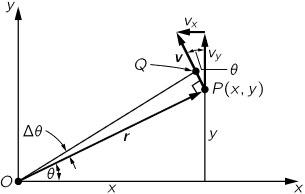
\includegraphics[width=0.3\textwidth]{pic1.png}
    \caption{二维旋转运动学}
    \end{figure}
    \begin{align}
    \Delta x&=-PQ \sin\theta=-r\Delta\theta \frac{y}{r}=-y\Delta\theta \\
    \Delta y&=+x\Delta\theta
    \end{align}

    关联的坐标正好交换了!
    \end{frame}

\subsection{速度关系}
    \begin{frame}
    \frametitle{速度关系}
    然后我们等式两边同时除以$\Delta t$,根据速度的定义即可得到:
    \begin{equation}
        v_x=-\omega y,\quad  v_y=+\omega x
    \end{equation}
    然而,当我们求出速度的大小时,这种奇怪的现象就消失了!
    \begin{equation}
    v=\sqrt{v_x^2+v_y^2}=r\omega
    \end{equation}
    \end{frame}

\subsection{通常推导}
    \begin{frame}
    \frametitle{通常推导}
    所以在通常的课本上,我们推导时就不会发现这种奇妙的事情。
    \begin{block}{结论}
    \begin{align}
    |\Delta \mathbf{r}|&=r\Delta\varphi \\
    |\Delta \mathbf{v}|&=\lim_{\Delta t \rightarrow 0} \frac{|\Delta \mathbf{r}|}{\Delta t}= r \lim_{\Delta t \rightarrow 0}\frac{|\Delta \varphi|}{\Delta t}= \omega r
    \end{align}
    \end{block}
    \end{frame}

\end{CJK}
\end{document}